%%=============================================================================
%% Voorbereiding op het onderzoek
%%=============================================================================

\chapter{Dimensioneel model: data warehousing}
\label{ch:dimmodel}
In dit hoofdstuk wordt een data warehouse opgebouwd aan de hand van het dimensioneel modelleren. Net zoals bij het Data Vault model, moet hier alles geconfigureerd worden zodat een verbinding mogelijk is vanuit een rapporteringsomgeving.

\section{Overzicht datamodel}
\begin{figure}[h]
	\centering
	\includegraphics[scale=0.5]{../images/Dimensioneelmodel.png}
	\caption{Voorstelling van het dimensioneel model (gemaakt via Lucidchart.com).}
	\label{fig:dmdm}
\end{figure}

In dit datamodel worden de dimensions voorgesteld als de blauwe entiteiten. Deze bevatten de beschrijvende data die iets meer vertellen over de ''facts''. De business key wordt gebruikt als attribuut die de relatie legt naar de facts-table (die wordt voorgesteld in het rood). In dit model worden geen gegevens opgeslagen die meer vertellen over de oorsprong van de data, tevens wordt de historiek van de data niet bijgehouden.

\section{Staging area}
In de architectuur van Data Vault, is al reeds een staging area toegevoegd die alle informatie ongemanipuleerd bijhoudt. Voor dit onderdeel van het onderzoek zal de laag niet opnieuw worden toegevoegd, maar zal er gebruik gemaakt worden van de eerder toegevoegde laag (zie sectie \ref{sec:stagareadv}).

\section{Opbouw data warehouselaag}
In deze sectie wordt de data warehouselaag opgebouwd. In tegenstelling tot Data Vault wordt alle data in deze laag weggeschreven, inclusief de business logica die berekend moet worden. De benodigde data wordt opgehaald uit de staging area.
\subsection{ETL}
Voor er data marts kunnen gemaakt worden, dienen de tabellen in de data warehouselaag gevuld worden. In dit ETL-proces wordt een onderscheid gemaakt tussen 2 soorten entiteiten: dimentions en facts. Hiervoor dienen dus twee soorten ETL-processen opgesteld te worden. In deze subsectie wordt voor beiden een voorbeeld weergegeven van zo'n proces.

\subsubsection{Dimensions}
Bij het inladen van de dimensions bij het dimensioneel model, moeten er nooit berekeningen uitgevoerd worden, aangezien deze de beschrijvende data bevatten over de facts. Wel kan de data in dit proces gecleaned en gemanipuleerd worden om een betere structuur te krijgen. 

\begin{figure}[h]
	\centering
	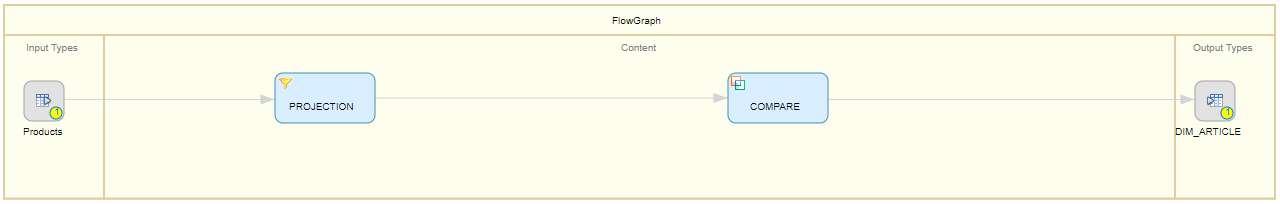
\includegraphics[scale=0.5]{../images/DM_FG_dim.png}
	\caption{Voorstelling van het ETL-proces bij een dimension (SAP SDI).}
	\label{fig:DM_FG_dim}
\end{figure}

In figuur 8.2 wordt het ETL-proces voorgesteld bij het inladen van de data in de tabel DIM\_ARTICLE. Aangezien er enkel data moet ingeladen worden vanuit één enkele tabel, moet er geen JOIN gebeuren. Er kan dus onmiddellijk begonnen worden met het transformeren van de data in PROJECTION. 

\begin{itemize}
	\item \textbf{ARTICLE\_ID (PK):} In dit attribuut wordt PRODUCT\_ID overgenomen van de brondata.
	\item \textbf{ARTICLE\_NAME:} In dit attribuut wordt PRODUCT\_DESCRIPTION overgenomen van de brondata.
\end{itemize} 

In de stap COMPARE wordt vergeleken of de nieuwe record al aanwezig is in de databank. Indien dit niet het geval is, wordt deze toegevoegd, anders wordt de record in de databank met dezelfde key overschreven. Bij het dimensioneel model wordt geen historiek bijgehouden van gegevens.

\subsubsection{Facts}
Bij een fact tabel, wordt de key van elke dimension bijgehouden. Alle sleutels samen vormen een composite key die dan geldt als primary key. Dit zorgt voor een zekere complexiteit bij het opbouwen van het ETL-proces. In dit proces worden ook de berekeningen uitgevoerd die nodig zijn voor het uitrekenen of de KPI wel/niet bereikt is.

\begin{figure}[h]
	\centering
	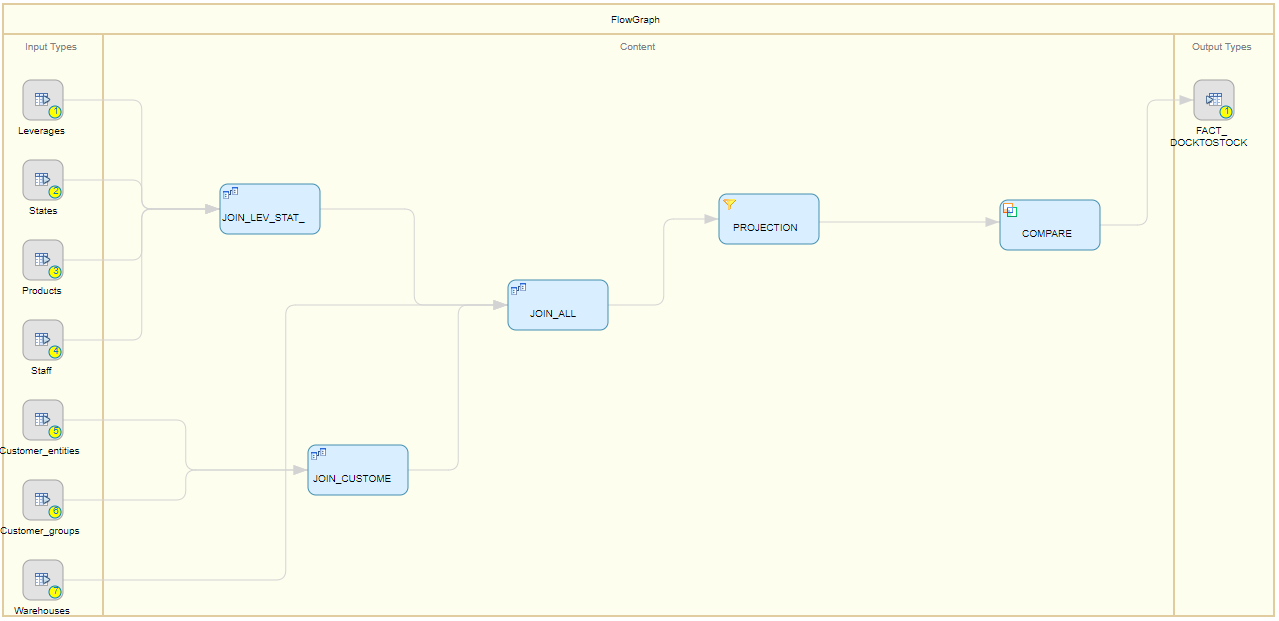
\includegraphics[scale=0.5]{../images/DM_FG_fact.png}
	\caption{Voorstelling van het ETL-proces bij een fact (SAP SDI).}
	\label{fig:DM_FG_fac}
\end{figure}

In stap 1 (JOIN\_LEV\_STAT\_PROD\_STAFF) wordt de data van de tabellen Leverages, States, Products en Staff samengevoegd op basis van de aanwezige attributen in de source tabel Leverages. Alleen de benodigde data wordt meegenomen naar de volgende stap. Bij JOIN\_CUSTOMER wordt tussen de tabellen Customer\_Entities en Customer\_Groups een relatie gelegd. Om uiteindelijk alles samen te voegen tot één geheel, wordt er een finale join (JOIN\_ALL) aangelegd. Hierbij wordt de data van JOIN\_LEV\_STAT\_PROD\_STAFF, JOIN\_CUSTOMER en Warehouses gecombineerd die kan gebruikt worden in de volgende stappen.

Vervolgens wordt de benodigde data berekend. Volgende transformaties worden toegepast:

\begin{itemize}
	\item \textbf{STAFF\_ID (PK):} In dit attribuut wordt STAFF\_ID overgenomen van de brondata.
	\item \textbf{ARTICLE\_ID (PK):} In dit attribuut wordt PRODUCT\_ID overgenomen van de brondata.
	\item \textbf{STATUS\_ID (PK):} In dit attribuut wordt STATUS\_ID overgenomen van de brondata.
	\item \textbf{WAREHOUSE\_ID (PK):} In dit attribuut wordt WAREHOUSE\_ID overgenomen van de brondata.
	\item \textbf{LABO\_ENTITY\_ID (PK):} In dit attribuut wordt LABO\_ENTITY\_ID overgenomen van de brondata.
	\item \textbf{LEVERAGE\_ID (PK):} In dit attribuut wordt LEVERAGE\_ID overgenomen van de brondata.
	\item \textbf{PALLET\_ID (PK):} In dit attribuut wordt PALLET\_ID overgenomen van de brondata.
	\item \textbf{LABO\_GROUP\_ID (PK):} In dit attribuut wordt LABO\_GROUP\_ID overgenomen van de brondata.
	\item \textbf{ARTICLE\_QUANTITY :} In dit attribuut wordt PRODUCT\_QUANTITY overgenomen van de brondata.
	\item \textbf{TOTAL\_STOCKED :} In dit attribuut wordt het getal '1' opgeslagen. Zo kan er na de aggregatie een deling uitgevoerd worden om een bepaald percentage uit te rekenen. Tevens zorgt dit ook voor een duidelijke naam voor de business.
	\item \textbf{SECONDS\_TO\_LATE :} Indien het verschil tussen STOCK\_TIJD en DOCK\_TIJD kleiner is dan 86400 seconden (24u), dan is het resultaat 0. Indien dat verschil groter is dan 86400 seconden, dan wordt het verschil tussen STOCK\_TIJD en DOCK\_TIJD weergegeven.
	\item \textbf{SECONDS\_BETWEEN\_DOCK\_AND\_STOCK :} In dit attribuut wordt het verschil tussen STOCK\_TIJD en DOCK\_TIJD weergegeven.
	\item \textbf{STOCKED\_WITHIN\_12HOURS\_QUANTITY :} Indien de pallet gestockeerd werd binnen de 12 uur tijd, dan is de waarde van dit attribuut 1, anders 0.
	\item \textbf{STOCKED\_WITHIN\_16HOURS\_QUANTITY :} Indien de pallet gestockeerd werd binnen de 16 uur tijd, dan is de waarde van dit attribuut 1, anders 0.
	\item \textbf{STOCKED\_WITHIN\_24HOURS\_QUANTITY :} Indien de pallet gestockeerd werd binnen de 24 uur tijd, dan is de waarde van dit attribuut 1, anders 0.
\end{itemize} 

Nadat alle transformaties en berekeningen zijn toegepast, worden de toegekomen waardes vergeleken met de huidige waardes van de destination table. Er wordt vergeleken op basis van de composite key. Indien de waarde al in de database aanwezig is, wordt deze overschreven, anders wordt deze toegevoegd aan de dataset.

\section{Opbouw data mart}
Nadat alle tabellen in het dimensioneel model zijn aangevuld, kan er een data mart aangemaakt worden voor de opgestelde KPI. Dit gebeurt gelijkaardig zoals bij het Data Vault model. Er zal een sterschema aangemaakt worden waarbij alle dimensions verbonden worden met de fact tabel. Hierop kan dan verbonden worden vanuit een rapporteringsomgeving. 

\begin{figure}[h]
	\centering
	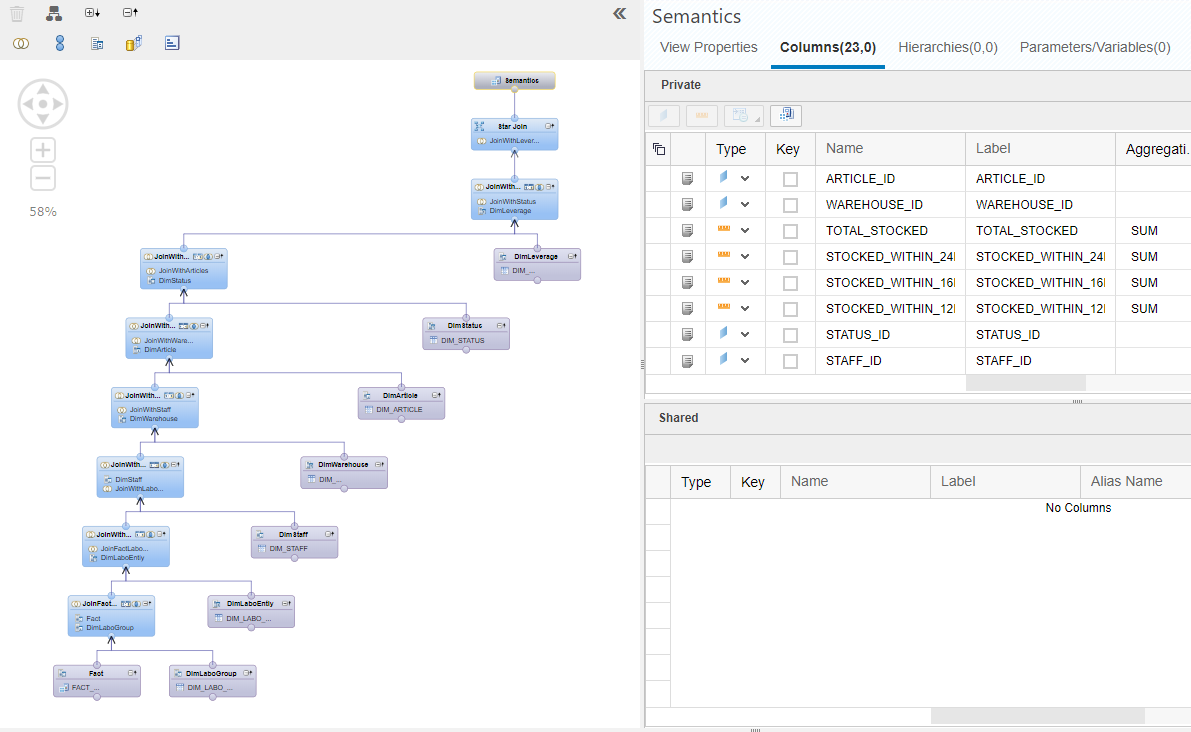
\includegraphics[scale=0.5]{../images/DM_FG_datamart.png}
	\caption{Sterschema opgesteld in SAP voor het dimensioneel model.}
	\label{fig:dmdmart}
\end{figure}
